%!TEX program = xelatex

\documentclass[compress]{beamer}
%--------------------------------------------------------------------------
% Common packages
%--------------------------------------------------------------------------

\definecolor{links}{HTML}{663000}
\hypersetup{colorlinks,linkcolor=,urlcolor=links}

\usepackage[english]{babel}
\usepackage{pgfpages} % required for notes on second screen
\usepackage{graphicx}

\usepackage{multicol}

\usepackage{tabularx,ragged2e}
\usepackage{booktabs}

\usetheme{hri}

% Display the navigation bullet even without subsections
\usepackage{remreset}% tiny package containing just the \@removefromreset command
\makeatletter
\@removefromreset{subsection}{section}
\makeatother
\setcounter{subsection}{1}


\newcommand{\source}[2]{{\tiny\it Source: \href{#1}{#2}}}

\usepackage{tikz}
\usetikzlibrary{mindmap,backgrounds,positioning,calc,patterns}

\graphicspath{{figs/part5/}}

\title{ROCO318 \newline Mobile and Humanoid Robots}
\subtitle{Part 5 - Bipedal Robots}
\date{}
\author{Séverin Lemaignan}
\institute{Centre for Neural Systems and Robotics\\{\bf Plymouth University}}

\begin{document}

\licenseframe{github.com/severin-lemaignan/module-mobile-and-humanoid-robots}

\maketitle

\videoframe[0.56]{figs/part5/robocup-2016-nao-devils-b-human.avi}
\videoframe[0.56]{figs/part5/darpa-humanoid-robots-falling.mp4}

\begin{frame}{Why walking robots?}
    \begin{columns}
        \begin{column}{0.5\linewidth}
    Mobility

    \begin{itemize}

        \item Wheeled robots only function on prepared surfaces (e.g. roads, rails,
            \ldots{}).
        \item Legged robots can negotiate difficult terrain, which wheeled robots
            cannot reach.
    \end{itemize}

    Understanding

    \begin{itemize}

        \item Understanding animal legged motion.
    \end{itemize}
            
        \end{column}
        \begin{column}{0.5\linewidth}
            \begin{center}
                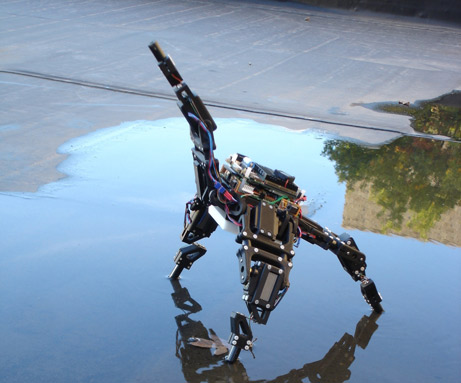
\includegraphics[width=0.8\linewidth]{image1}

                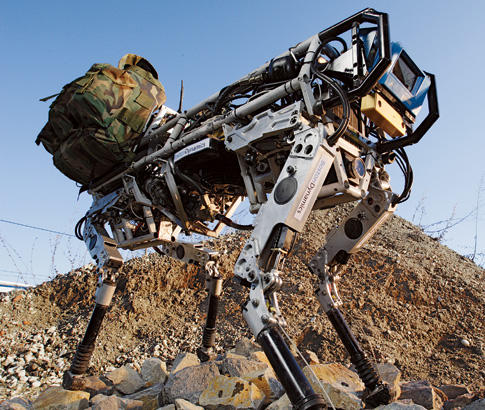
\includegraphics[width=0.8\linewidth]{image2}
            \end{center}
        \end{column}
    \end{columns}

\end{frame}

\begin{frame}{Why bipedal walking?}
    \begin{columns}
        \begin{column}{0.5\linewidth}

    Because humanoid robots only have two legs.

    \begin{itemize}

        \item Better mobility over rough terrain.
        \item Active suspension that stabilises the load.
        \item Overcoming obstacles, i.e. avoiding or moving over or under obstacles.
    \end{itemize}

    Humans relate to humanoid robots much more readily.

    \begin{itemize}

        \item Human--Robot Interaction.
    \end{itemize}
            
        \end{column}
        \begin{column}{0.5\linewidth}
            \begin{center}
                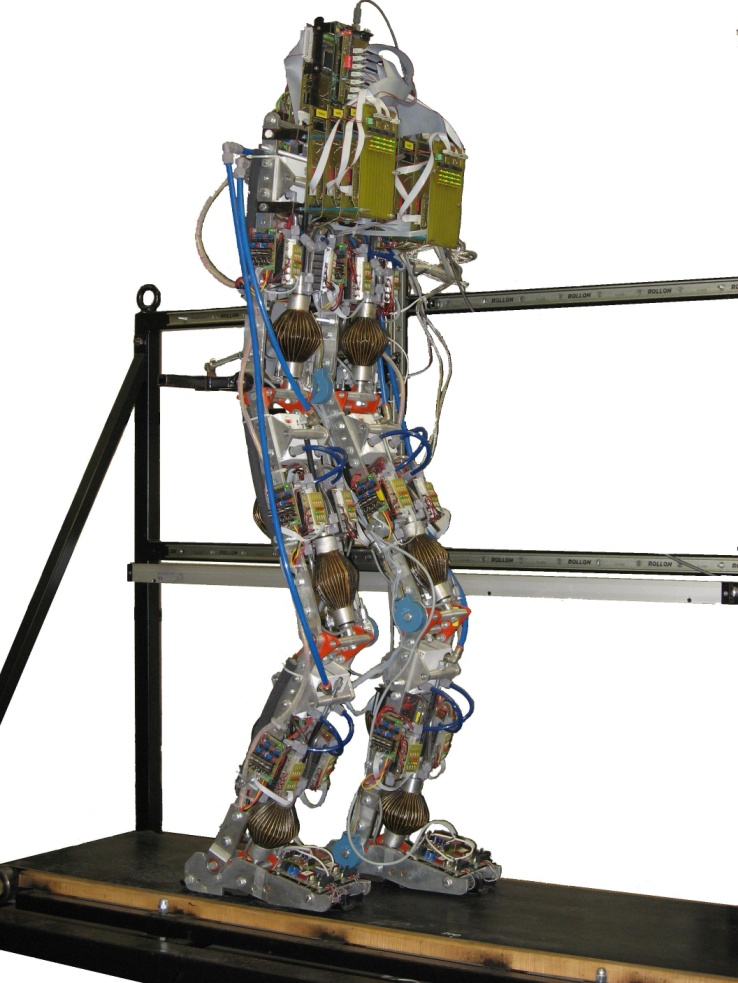
\includegraphics[width=0.8\linewidth]{lucy}

    \source{http://lucy.vub.ac.be/}{Lucy, VUB}
            \end{center}
        \end{column}
    \end{columns}

\end{frame}

\begin{frame}{Why bipedal walking?}

    \begin{columns}
        \begin{column}{0.5\linewidth}
    As a tool for understanding human gait disorders

    Active prosthetics

    \begin{itemize}

        \item E.g.
            \href{https://www.ted.com/talks/hugh_herr_the_new_bionics_that_let_us_run_climb_and_dance?language=en}{Hugh
            Herr's prothetic legs}.
    \end{itemize}

    Exoskeletons

    \begin{itemize}

        \item E.g. \href{http://www.youtube.com/watch?v=2Ysb-Oko3Bg}{Cyberdine HAL}
    \end{itemize}

    The human environment has been adapted profoundly to bipedal locomotion.

    \textbf{Just because it's cool!}
            
        \end{column}
        \begin{column}{0.5\linewidth}
            \begin{center}
                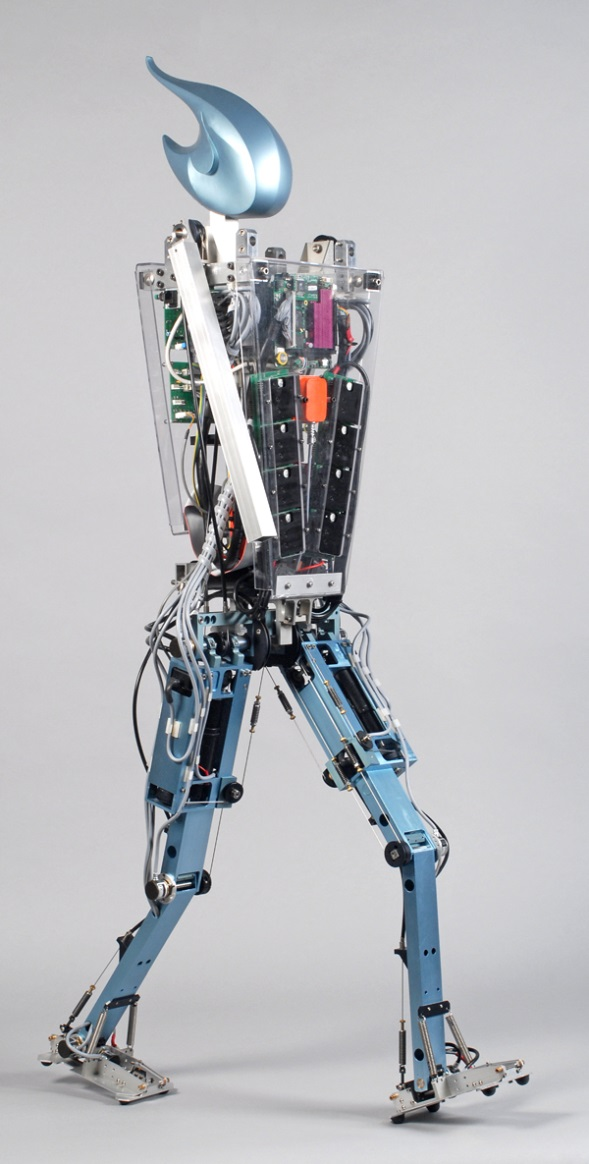
\includegraphics[height=0.6\paperheight]{flame}
    
                \source{http://www.3me.tudelft.nl/en/about-the-faculty/departments/biomechanical-engineering/research/dbl-delft-biorobotics-lab/bipedal-robots/}{Flame, TU Delft}
            \end{center}
        \end{column}
    \end{columns}


\end{frame}

\begin{frame}{Speed of robots}

    \begin{center}
       \footnotesize 
\begin{tabular}{p{2.6cm}p{2.6cm}p{2.6cm}p{2.6cm}}
\video[1.2]{1.8cm}{figs/part5/walking_person.mp4} & 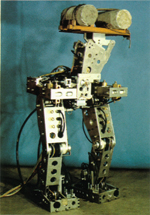
\includegraphics[height=2.2cm]{image7} & 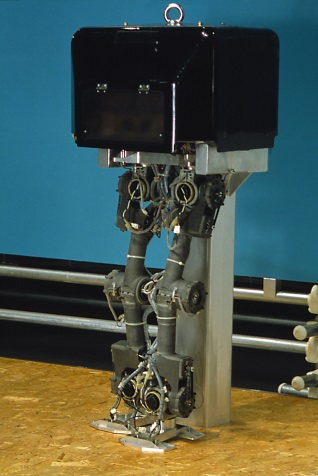
\includegraphics[height=2.2cm]{image8} & \\
    Walking person \emph{$\pm$5km/h} & WL-5 ('70) \emph{45s/step}  & E2 ('91) \emph{1.2km/h} & \\
 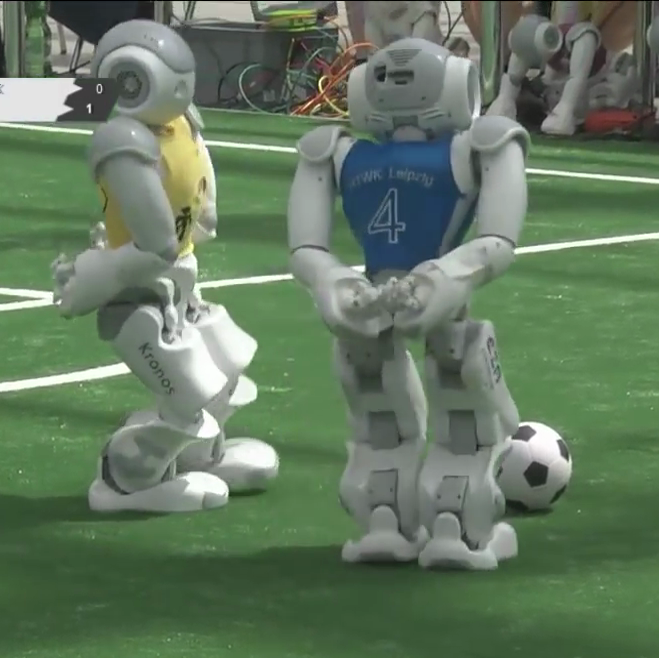
\includegraphics[height=2.2cm]{nao-robocup} & 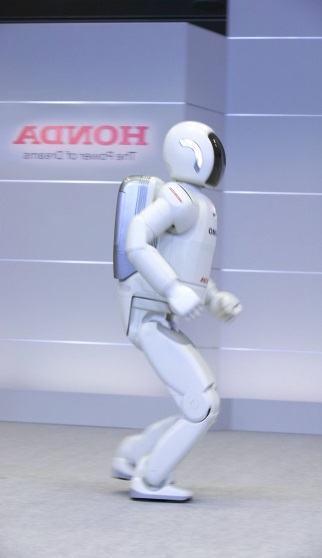
\includegraphics[height=2.2cm]{image6} & 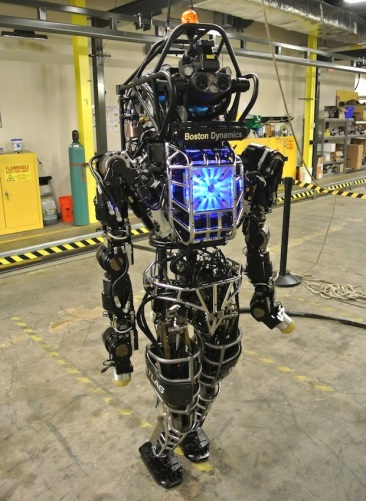
\includegraphics[height=2.2cm]{image11} & 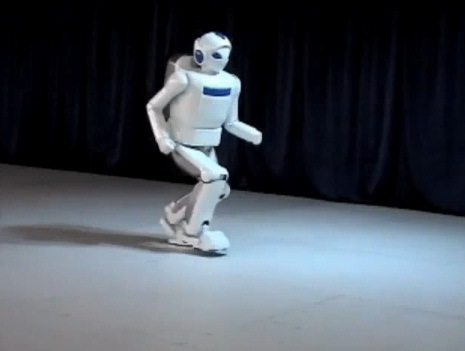
\includegraphics[height=2.2cm]{image10} \\
    Nao \emph{1.6km/h}                 & Asimo \emph{6km/h}             & Atlas robot  \emph{7km/h} & Partner \emph{7km/h}
\end{tabular}

    \end{center}

    \pause
    Biped robot speed is often expressed as body lengths per second, to make
    comparison with different sized robots possible.

\end{frame}

\imageframe[caption=Usain Bolt WR 100m: 36.8km/h]{bolt}

\begin{frame}{What is bipedal walking?}

    \textbf{Walking}: when two feet are in contact with the ground at some point in the gait
    cycle.

    \textbf{Running}: when only one foot touches the ground at any point in the
    gait cycle.

    A \textbf{gait cycle} starts with an initial contact of one foot with the
    ground, and ends at the next contact of the same foot with the ground.

    Two phases to a gait cycle:

    \begin{itemize}

        \item \textbf{Stance phase} --when the foot is in contact with the ground
            (also called \emph{support phase});
        \item \textbf{Swing phase} --when the foot is lifted of the ground.
    \end{itemize}

\end{frame}

\begin{frame}{Robot walking - Active}

    \textbf{Active Walk}

    \begin{itemize}

        \item An active walk is when the robot is internally powered. This is
            usually through electrical servos, pneumatics or hydraulics.
        \item Versatile
        \item Continuous high bandwidth control
        \item Fully actuated, resulting in high energy consumption
        \item \href{http://www.youtube.com/watch?v=cHJJQ0zNNOM}{BigDog}
            (\href{http://www.youtube.com/watch?v=VXJZVZFRFJc}{2},
            \href{http://www.youtube.com/watch?v=-Bi-tPO0OPs}{talk}),
            \href{http://www.youtube.com/watch?v=Q3C5sc8b3xM}{Honda Asimo},
            \href{http://www.youtube.com/watch?v=KaIfZW7vCGI\&feature=related}{Bioloid},
            \ldots{}
    \end{itemize}

\end{frame}

\begin{frame}{Robot walking - Passive}

    \textbf{Passive Walk}

    \begin{itemize}

        \item A passive walk is when a robot is not internally powered. This is
            usually driven by an initial push or through gravity (downhill)
        \item Fixed walking speed, no starting, stopping or turning
        \item No actuation (slope needed)
        \item No control
        \item Very low energy consumption
        \item \href{http://www.youtube.com/watch?v=N64KOQkbyiI}{Passive walker
            example},
            \href{http://www.youtube.com/watch?v=CK8IFEGmiKY\&NR=1}{Nagoya U.}
    \end{itemize}

\end{frame}

\begin{frame}{Robot walking - Static}

    \textbf{Static Walk}

    \begin{itemize}

        \item A static walk is when the robot is always \textbf{balanced. If the
            robot was to stop at any point in the gait cycle then it would not
            fall over.}
        \item Control is easy.
        \item Movements are slow.
        \item \href{http://www.youtube.com/watch?v=NbnELOZbsls\&feature=related}{Aldebaran
            Nao} (\href{http://www.youtube.com/watch?v=3aOuQ1_e--k}{not always}),
            \href{http://www.youtube.com/watch?v=cYo9Whssla8}{LittleDog}
    \end{itemize}

\end{frame}

\begin{frame}{Robot walking - Dynamic}

    \textbf{Dynamic Walk}

    \begin{itemize}

        \item A dynamic walk when the robot is not \textbf{balanced. If the robot
            was to stop at any point in the gait cycle then it would fall over.
            Controlled falling.}
        \item Control is hard.
        \item Fast(er) motion.
        \item Honda Asimo, \href{http://www.youtube.com/watch?v=KLepY1AsaRk}{Cornell
            walkers}, Delft walkers,
            \href{http://www.youtube.com/watch?v=diaZFIUBMBQ}{Schaft robot}
    \end{itemize}

\end{frame}

\begin{frame}{Static/Dynamic}

    Humanoid Robotics Project (HRP2) robot (Japan, 1997-)

    \vspace{1em}
    \begin{columns}
        \begin{column}{0.5\linewidth}
    Static walking

            \video{\linewidth}{figs/part5/hrp2-1.mp4}
            
        \end{column}
        \begin{column}{0.5\linewidth}
    Dynamic walking

            \video{\linewidth}{figs/part5/hrp2-2.mp4}
        \end{column}
    \end{columns}



\end{frame}

\begin{frame}{Robot walking (3)}

    \begin{tikzpicture} 
        [>=latex,label/.style={align=center,font=\footnotesize},scale=0.8]


        \draw[ultra thick,->] (-5,0) -- (5,0);
        \draw[ultra thick,->] (0,-4) -- (0,4);

    \end{tikzpicture}

    \begin{itemize}

        \item Combinations
    \end{itemize}

    \textbf{Active static}


    Always in balance, with energy input.
    \textbf{Active dynamic}

    Controlled falling, with energy input.
    \textbf{Passive static}


    Does not walk. A brick.

    \textbf{Passive dynamic}

    Controlled falling, no energy input to the system.

    \emph{Passive/Active}

    \emph{Static/ Dynamic}

\end{frame}

\begin{frame}{Energy consumption}

    \begin{center}
        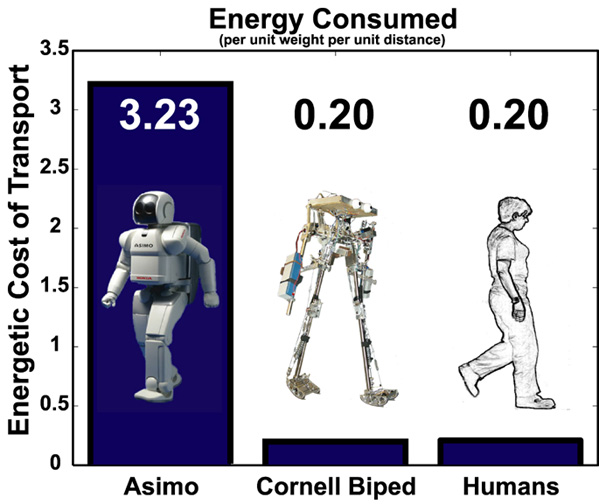
\includegraphics[width=0.8\linewidth]{image14}
    \end{center}
\end{frame}

\begin{frame}{People}

    \begin{center}
        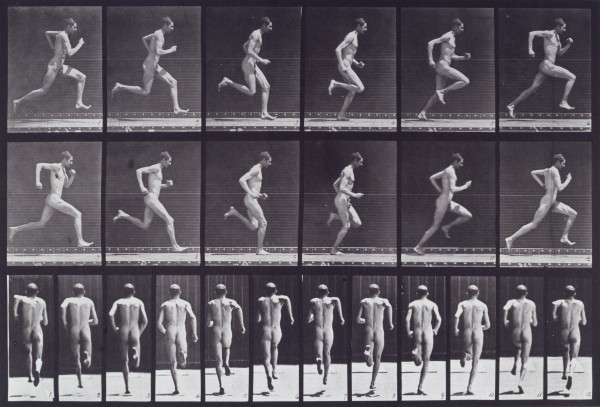
\includegraphics[width=0.8\linewidth]{image15}

    \emph{\textbf{Eadweard Muybridge}}
    \end{center}

\end{frame}

\begin{frame}{How do people walk?}

    Human Perspective

    \begin{itemize}

        \item Humans use a mixture of active/passive and static/dynamic walking.
        \item Walking requires generating energy (active) but the energy is also
            conserved where possible (passive).
        \item Humans can balance (static) although this requires more energy
            therefore they use an efficient unbalanced gait (dynamic).
    \end{itemize}

    Robot Perspective

    \begin{itemize}

        \item Most robot research has focused on either an active static gait, an
            active dynamic gait or a passive dynamic gait.
    \end{itemize}

\end{frame}

\begin{frame}{Actuation}

    Hydraulics

    \begin{itemize}

        \item Pressurised liquid.
        \item Bigdog and \href{http://www.youtube.com/watch?v=QRbvNL1PHKg}{Petman}.
    \end{itemize}

    Pneumatics

    \begin{itemize}

        \item Air powered: high energy, powerful.
        \item Inherently compliant.
    \end{itemize}

    DC motors

    \begin{itemize}

        \item Can be combined with spring to have compliant motors.
        \item \href{http://www.youtube.com/watch?v=XVYsqv3sLew}{iCub walking}.
    \end{itemize}

    Servo motors

    \begin{itemize}

        \item DC motors with gears and positioning electronics
    \end{itemize}

\end{frame}

\section{Servo motor powered humanoid robots}

\begin{frame}{What is a servo motor?}

    \begin{columns}
        \begin{column}{0.5\linewidth}
    A servo motor is a combination of a DC motor, gearing and a position
    measurement.

    \begin{itemize}

        \item Position measurement is used for negative feedback to decrease error
            between current position and demanded position.
    \end{itemize}

            
        \end{column}
        \begin{column}{0.5\linewidth}
            \begin{center}
                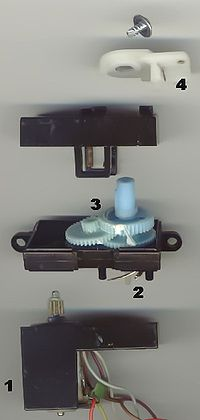
\includegraphics[width=0.8\linewidth]{image17}

    \source{http://en.wikipedia.org/wiki/Servomechanism}{RC servo motor (Wikipedia)}
            \end{center}
        \end{column}
    \end{columns}

    \begin{center}
        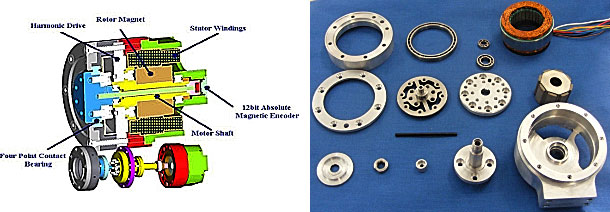
\includegraphics[width=0.8\linewidth]{image18}
    \source{http://www.iit.it/en/advanced-robotics/projects/the-lower-body-of-the-child-humanoid-robot-icub.html}{iCub motor arrangement, can be used in servo mode}

    \end{center}
\end{frame}

\begin{frame}{Why servo motors?}

    Large percentage of humanoid robots use servo motors

    \begin{itemize}

        \item Traditional method of powering a robot. The vast majority of
            industrial robots use motors to control the movement of the robots.
        \item Large knowledge base for servo motor control.
        \item Can be scaled for larger or smaller robots.
        \item Powered by electricity via a fixed or portable power supply.
        \item Accurate control of position.
        \item Large range of movement.
        \item Good power to weight ratio.
        \item Good speed characteristics.
        \item Cost effective solution.
    \end{itemize}

\end{frame}

\begin{frame}{Humanoids and servos}

    From industrial robots to humanoid robots

    \begin{itemize}

        \item Many of the first humanoid robots were developed from existing
            technology used in industrial robots.
        \item Car manufacturers use large numbers of industrial robots and were
            amongst the first companies to invest heavily in the development of
            new technologies to produce a humanoid robot.
    \end{itemize}

\end{frame}

\begin{frame}{Examples}

    Humanoid Robots Using Servo Motors

    \begin{itemize}

        \item Honda Asimo
        \item Toyota humanoid
        \item Aldebaran Nao
        \item Team Osaka football player
        \item Bioloid
    \end{itemize}

    \begin{center}
        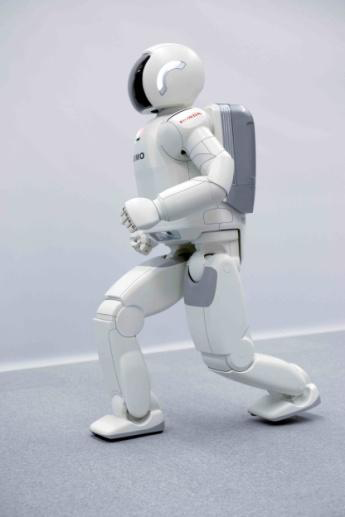
\includegraphics[width=0.2\linewidth]{image19}
        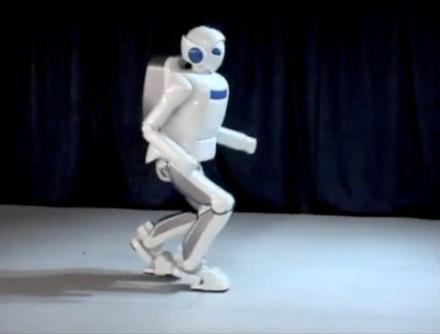
\includegraphics[width=0.2\linewidth]{image20}
        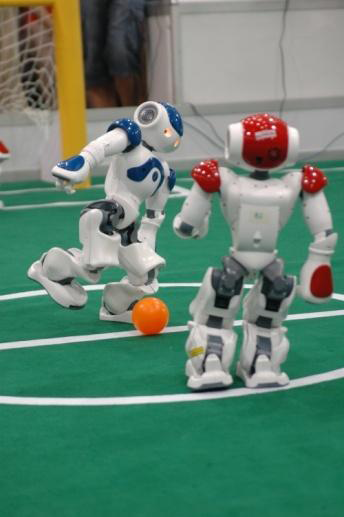
\includegraphics[width=0.2\linewidth]{image21}
        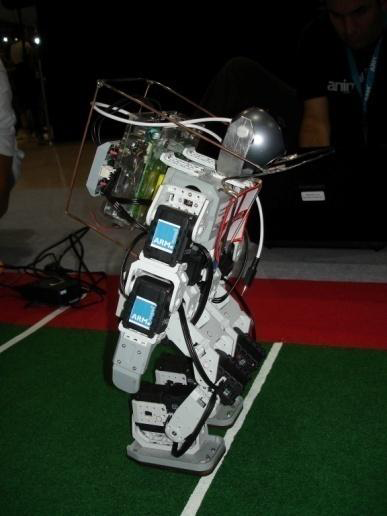
\includegraphics[width=0.2\linewidth]{image22}
        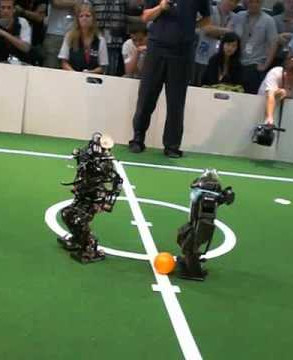
\includegraphics[width=0.2\linewidth]{image23}
    \end{center}
\end{frame}

\begin{frame}{Bioloid robot}

    \href{http://www.robotis.com/xe/bioloid_en}{Bioloid} Robot
    Specifications

    \begin{columns}
        \begin{column}{0.5\linewidth}
    \begin{itemize}

        \item Manufactured by Robotis in South Korea.
        \item Has 18 Degrees of Freedom (= motors).
        \item Designed to be reconfigured into different forms.
        \item Cost between £600 -£800.
        \item Robust.
        \item Easy to assemble.
        \item 40cm tall.
        \item Weighs 1.7Kg.
        \item Programmable.
        \item Safe.
    \end{itemize}
            
        \end{column}
        \begin{column}{0.5\linewidth}
            \begin{center}
                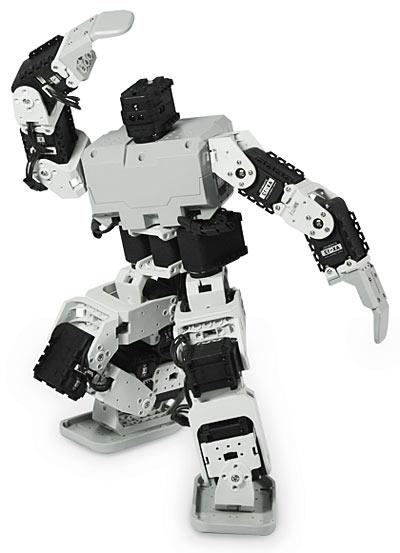
\includegraphics[width=0.8\linewidth]{image24}
            \end{center}
        \end{column}
    \end{columns}

\end{frame}

\begin{frame}{Bioloid robot (2)}

    Motors, brackets and comms module used for the Plymouth humanoids.

    Can be programmed in two ways

    \begin{itemize}

        \item Using an editor (RoboPlus)
        \item C (cross-compiled to Atmel processor assembly).
    \end{itemize}

    \begin{center}
        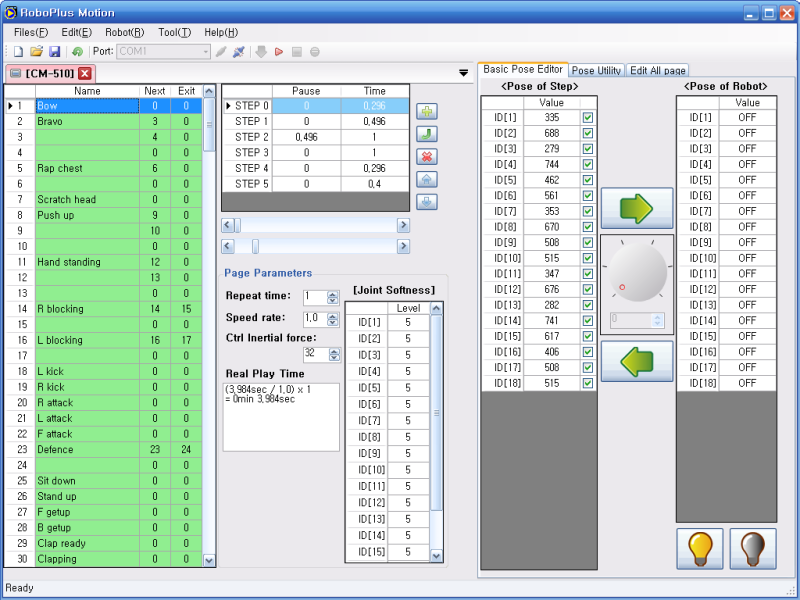
\includegraphics[width=0.8\linewidth]{image25}
    \end{center}
\end{frame}

\begin{frame}{Bioloid robot (3)}

    \begin{itemize}

        \item Difficult to create exact controlled movements such as walking.
        \item Takes a long time to manually enter the exact positions calculated for
            the robots.
        \item Restricted by the performance of the AX-12 servo motors.
        \item Compliance in the motors affects performance.
    \end{itemize}

    \begin{center}
        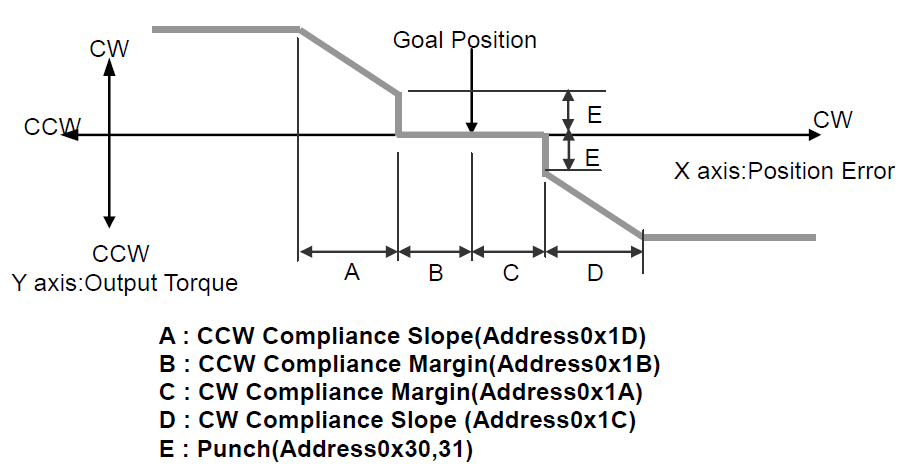
\includegraphics[width=0.8\linewidth]{image26}
    \end{center}
\end{frame}

\begin{frame}{AX-12+ Servo Motor}

    \begin{columns}
        \begin{column}{0.5\linewidth}
    AX-12+ Specifications

    \begin{itemize}

        \item Weight 55g.
        \item Has a maximum speed of 50 RPM at 10 volts.
        \item A maximum torque of 16.5 Kgf.cm or 1.62 Nm.
        \item Has a gear ratio reduction of 1/254.
        \item Operating angle of 300 degrees.
        \item Uses plastic gears.
        \item Programmable.
    \end{itemize}
            
        \end{column}
        \begin{column}{0.5\linewidth}
            \begin{center}
                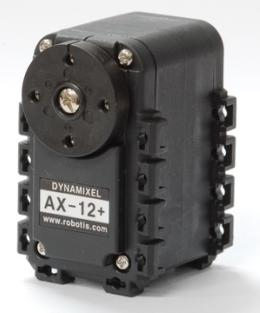
\includegraphics[width=0.8\linewidth]{image28}

                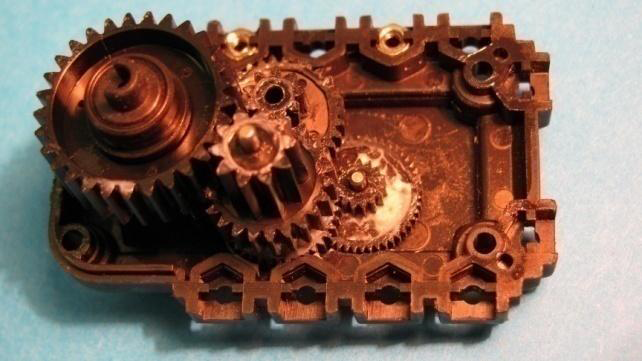
\includegraphics[width=0.8\linewidth]{image27}
            \end{center}
        \end{column}
    \end{columns}

\end{frame}

\begin{frame}{AX-12+ Servo Motor (2)}

    AX-12+ Servo Specifications

    \begin{itemize}

        \item AX-12 servo motor uses an AtmelMega8.
        \item Uses Serial RS232 communication at 128Hz or every 7.8 mS.
        \item Calculate the required position of the motor then send the speed and
            position for the motor.
    \end{itemize}

    \begin{center}
        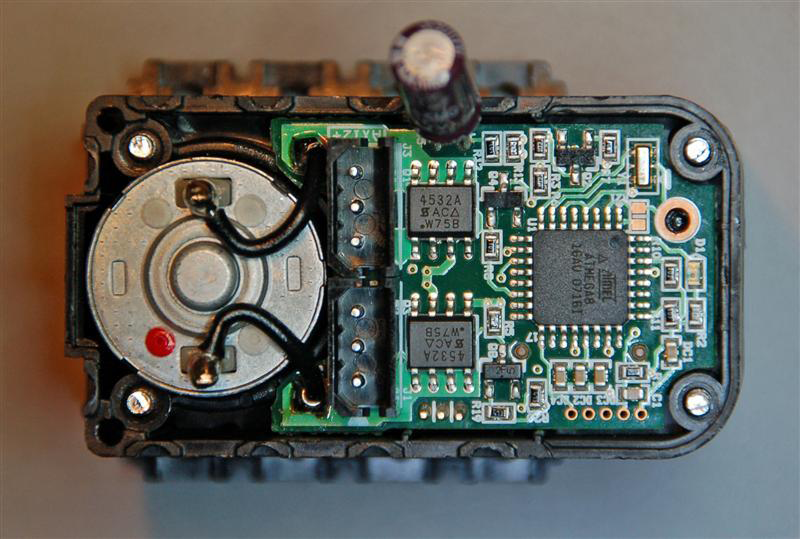
\includegraphics[width=0.4\linewidth]{image29}
        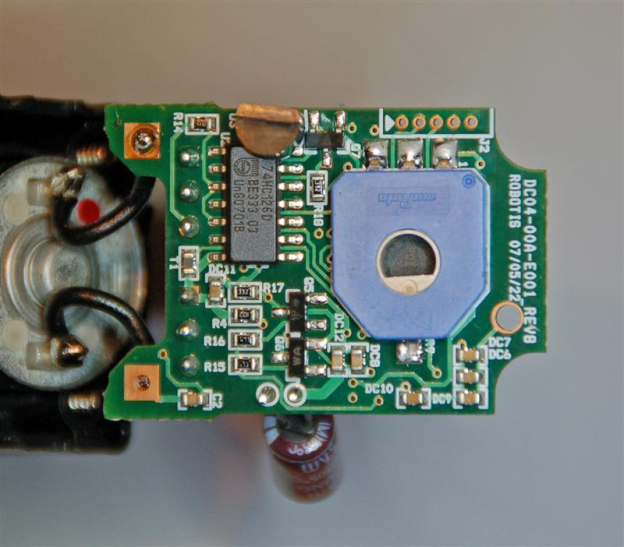
\includegraphics[width=0.4\linewidth]{image30}
    \end{center}
\end{frame}

\begin{frame}{Bioloid kinematics}

    Developing a robot gait.

    \begin{itemize}

        \item What gait pattern results in a robust and fast walk?
    \end{itemize}

    To answer to these questions the robot needs to be able to translate the
    movement in an world coordinate system (x, y, z) in to the angle of
    rotation for the motors.

    \begin{itemize}

        \item This is achieved by using inverse kinematics.
    \end{itemize}

    Forward kinematics is when given an angle of the rotation of the motors
    the position of the foot can be calculated in world coordinates.

\end{frame}

\begin{frame}{Bioloid kinematics (2)}

    \begin{itemize}

        \item Bioloid Kinematics -Simplified
    \end{itemize}

    \begin{center}
        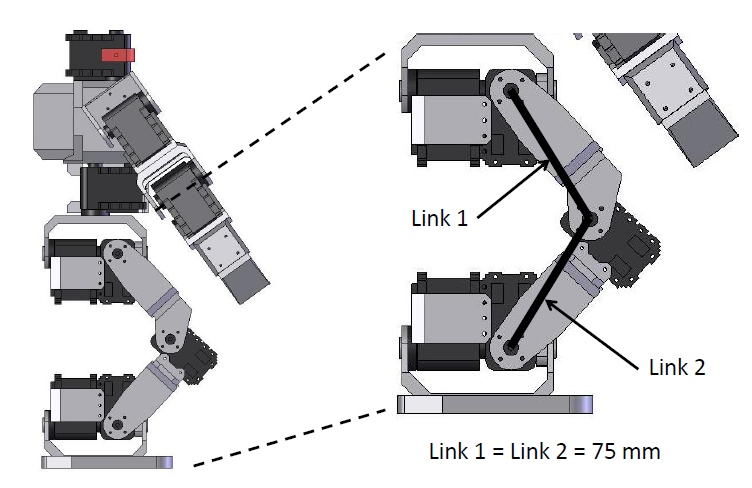
\includegraphics[width=0.8\linewidth]{image31}
    \end{center}
\end{frame}

\begin{frame}{Bioloid kinematics (3)}

    \begin{columns}
        \begin{column}{0.5\linewidth}
    \begin{itemize}

        \item Forward kinematics
        \item \emph{A1} and \emph{A2} are the angle of rotation, \emph{L1} and
            \emph{L2} are the length of the robot limbs
        \item Calculate the resultant position (\emph{XR}, \emph{YR}) first
            determine the X and Y component of each link and add these together.
    \end{itemize}
            
        \end{column}
        \begin{column}{0.5\linewidth}

            \begin{center}
                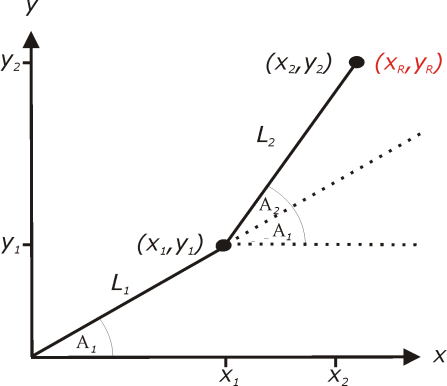
\includegraphics[width=0.8\linewidth]{image32}
            \end{center}

    sin \emph{A = opposite / hypotenuse}

    \emph{cosA = adjacent / hypotenuse}
        \end{column}
    \end{columns}


\end{frame}

\begin{frame}{Bioloid kinematics (4)}

    \begin{columns}
        \begin{column}{0.5\linewidth}

    \emph{XR= L1} cos\emph{(A1) + L2} cos\emph{(A1+ A2)}


    \emph{YR= L1} sin\emph{(A1) + L2} sin\emph{(A1+ A2)}
        \end{column}
        \begin{column}{0.5\linewidth}

            \begin{center}
                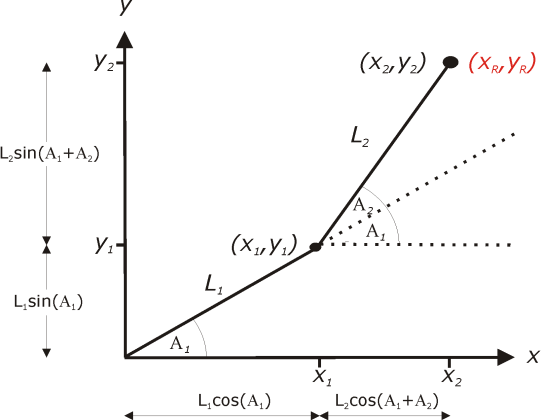
\includegraphics[width=0.8\linewidth]{image33}
            \end{center}
        \end{column}
    \end{columns}


\end{frame}

\begin{frame}{Bioloid kinematics (5)}

    Inverse kinematics

    \begin{align*}
        A_2 &= \cos^{-1} \left( \frac{x_R^2+y_R^2-L_1^2-L_2^2}{2L_1L_2} \right) \\
        A_1 &= \sin^{-1} \left( \frac{y_r}{\sqrt{x_R^2+y_R^2}} \right)-\sin^{-1}\left( \frac{L_2 \sin(A_2)}{\sqrt{x_R^2+y_R^2}} \right)
    \end{align*}

    \begin{columns}
        \begin{column}{0.5\linewidth}

    \begin{itemize}

        \item This is a geometric solution, more can be found in the document
            `\href{http://www.tribotix.info/Articles\&Tutorials/MathsforRobotics/Mathematics\%20required\%20for\%20Robotic\%20Motion.pdf}{Mathematics
            required for legged robotic motion}'.
    \end{itemize}
        \end{column}
        \begin{column}{0.5\linewidth}
            \begin{center}
                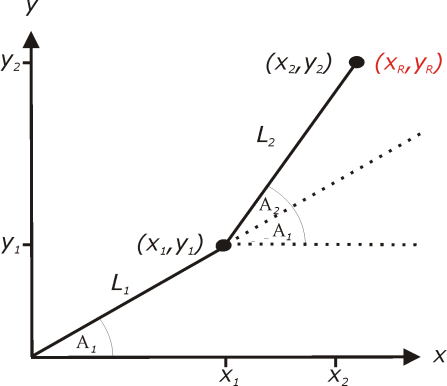
\includegraphics[width=0.8\linewidth]{image32}
            \end{center}
        \end{column}
    \end{columns}

\end{frame}

\begin{frame}{Servo-based humanoids}

    What do Servo Powered Humanoid Robots Have in Common?

    \begin{itemize}

        \item They never straighten their legs!
        \item Most servo powered robots either walk or run with their legs slightly
            bent.
        \item Produces an un-human like gait.
        \item Same for either statically of dynamically balanced robots.
        \item Results from the physical restrictions of using servo motors.
    \end{itemize}

    Use a simple kinematics model to prove why.

    An example of the problem can be shown using the Bioloid robot.

\end{frame}

\begin{frame}{Bioloid Gait Analysis}

    \begin{itemize}

        \item Starting with slightly bent knees means the knee servo motor is used
            more effectively resulting in the foot being lifted a greater distance
            and in a more controlled manner.
    \end{itemize}

    \begin{center}
        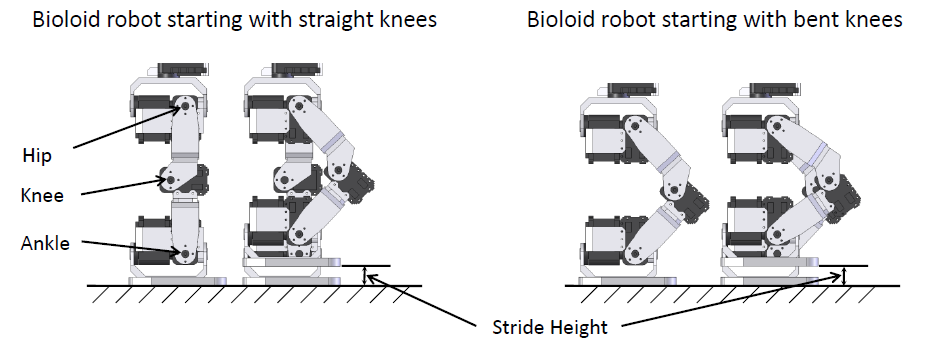
\includegraphics[width=0.8\linewidth]{image35}
    \end{center}
\end{frame}

\begin{frame}{Effort to lift foot 1cm?}

    \begin{columns}
        \begin{column}{0.5\linewidth}
    \textbf{Stretched leg}

        \begin{itemize}

            \item     Hip moves 21.0$^\circ$ knee moves 42.0$^\circ$
        \end{itemize}

            \begin{center}
                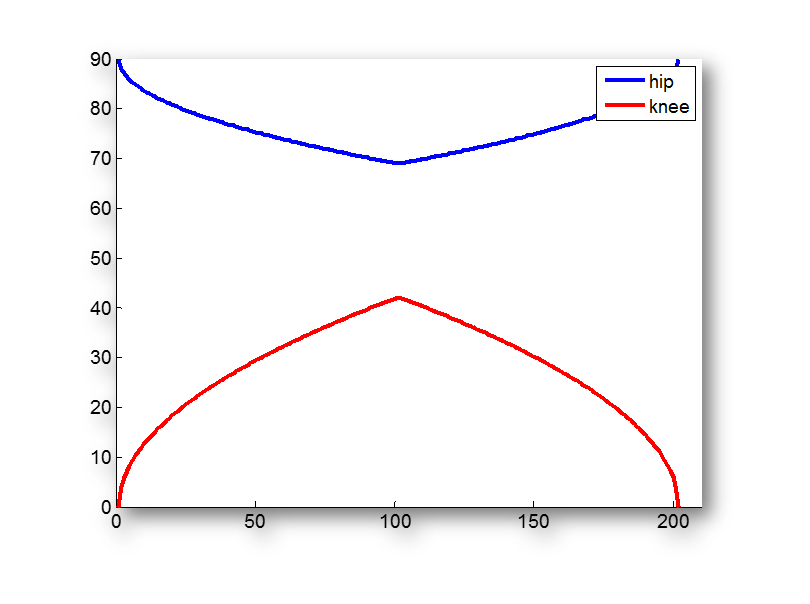
\includegraphics[width=0.8\linewidth]{graph1}
            \end{center}
            
        \end{column}
        \begin{column}{0.5\linewidth}

    \textbf{Bent knees}

        \begin{itemize}

            \item     Hip moves 8.9$^\circ$ knee moves 17.8$^\circ$
        \end{itemize}

            \begin{center}
                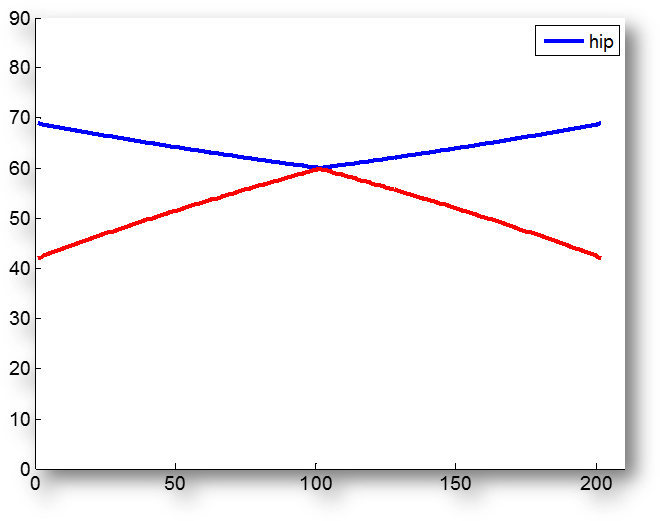
\includegraphics[width=0.8\linewidth]{graph2}
            \end{center}

        Much less angle change required for motors to lift foot same amount.
        \end{column}
    \end{columns}

\end{frame}

\begin{frame}{Effort to lift foot 1cm?}

    \begin{center}
        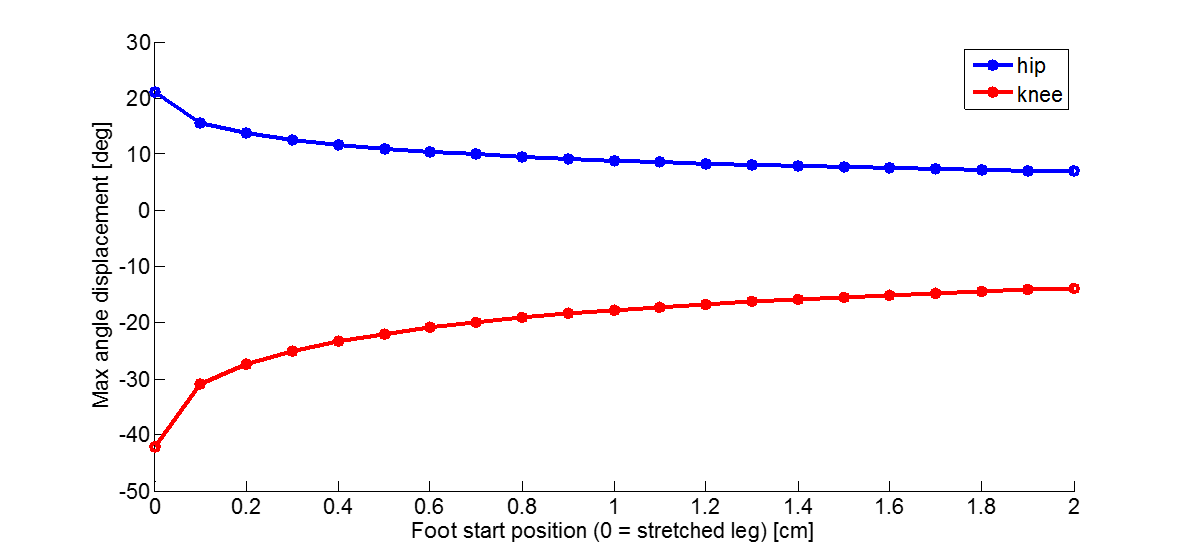
\includegraphics[width=0.8\linewidth]{graph3}
    \end{center}

    But further bending knees and hip has diminishing returns

    Starting with bent knees and hip requires less effort

    Starting from stretched legs requires the hip to flex 20$^\circ$ and the knee
    -42$^\circ$ to lift the foot 1 cm

\end{frame}

\begin{frame}{Bioloid Gait Analysis}

    What are the implications for the Bioloid robot gait?

    How often are the servo motors asked to move?

    \begin{itemize}

        \item Usually at 64Hz or every 15.6 ms.
    \end{itemize}

    Therefore what is the maximum angle they can rotate in that time.

    \begin{itemize}

        \item At 50 RPM = 300°/s -\textgreater{} 4.68° in 15.6 ms
    \end{itemize}

    As the height the foot is raised and the forward movement of the foot is
    increased the servo motors reach the limit of their speed.

    Above the maximum speed the gait will not be able to reach its
    calculated position. This could result in instability.

\end{frame}

\begin{frame}{Bioloid Gait Analysis (4)}

    Using a simple inverse kinematic solution for the Bioloid leg servos,
    the angle of rotation for a step height and length can be calculated.

    Given the update rate of the servo motors it is possible to calculate
    what is the maximum height and distance the foot can be moved. This
    gives a maximum possible theoretical speed for the robot to move.

    To improve the gait different motors speeds can be assessed.

    The gait generation pattern can be optimised for the motors.

    \begin{itemize}

        \item Currently the Bioloid uses the equation of an elipise to generate the
            gait pattern to follow.
    \end{itemize}

\end{frame}

\begin{frame}{Bioloid Gait Analysis -Summary}

    \begin{itemize}

        \item In order to reduce the computational cost for calculating the equation
            of an ellipse every 15.6 ms the solution in pre-calculated over a grid
            (75 mmx 70 mm) and stored in a look-up table.
    \end{itemize}

    \begin{center}
        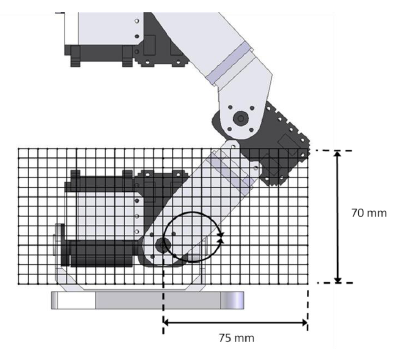
\includegraphics[width=0.8\linewidth]{image39}
    \end{center}
\end{frame}

\begin{frame}{Bioloid Dynamic Gait Generator (1)}

    \begin{itemize}

        \item There is also a Bioloid dynamic gate generator, which takes 10
            parameters to generate a series of robot poses.
    \end{itemize}

\end{frame}

\begin{frame}{Gait Generator -- parameters (1)}

    \begin{itemize}

        \item Swing -Hip movement (Sideways)
    \end{itemize}

    \begin{center}
        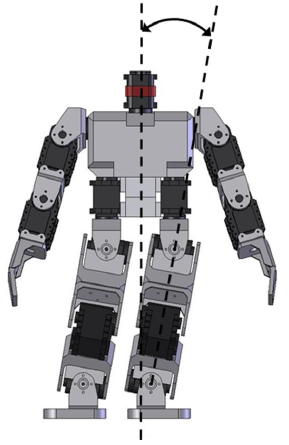
\includegraphics[height=0.5\paperheight]{bioloid-gait-1}
    \end{center}
\end{frame}

\begin{frame}{Gait Generator -- parameters (2)}

    \begin{itemize}

        \item Tilt -Hip (used to balance the robot)
    \end{itemize}
    \begin{center}
        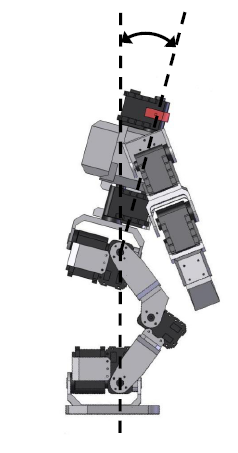
\includegraphics[height=0.5\paperheight]{bioloid-gait-2}
    \end{center}

\end{frame}

\begin{frame}{Gait Generator -- parameters (3)}

    \begin{itemize}

        \item Camber (Splaying legs)
    \end{itemize}
    \begin{center}
        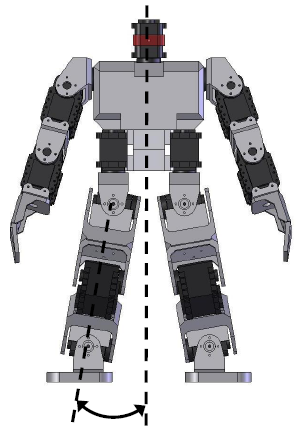
\includegraphics[height=0.5\paperheight]{bioloid-gait-3}
    \end{center}

\end{frame}

\begin{frame}{Gait Generator -- parameters (4)}

    \begin{itemize}

        \item Stride height (Foot lift)
    \end{itemize}
    \begin{center}
        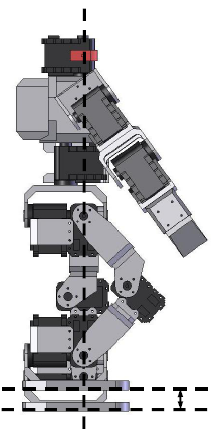
\includegraphics[height=0.5\paperheight]{bioloid-gait-4}
    \end{center}

\end{frame}

\begin{frame}{Gait Generator -- parameters (5)}

    \begin{itemize}

        \item Y-Offset (Starting position for knees)
    \end{itemize}
    \begin{center}
        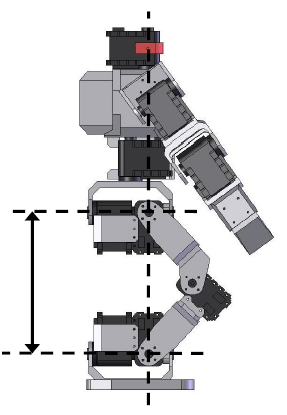
\includegraphics[height=0.5\paperheight]{bioloid-gait-5}
    \end{center}

\end{frame}

\section{Theories of walking}

\begin{frame}{Static walking}

    \begin{itemize}

        \item Based on keeping Centre of Gravity (COG) over the support polygon
    \end{itemize}

    \begin{center}
        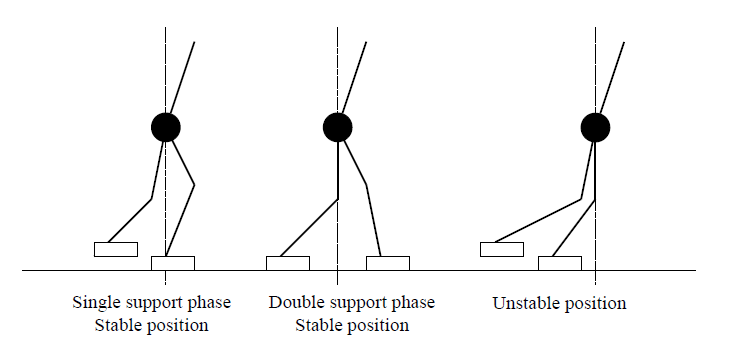
\includegraphics[width=0.8\linewidth]{image45}
        
    \source{http://www.diss.fu-berlin.de/diss/servlets/MCRFileNodeServlet/FUDISS_derivate_000000002504/05_Kapitel5.pdf;jsessionid=BB71E0C0242031B3A6B5F4E873C63233?hosts=}{Source}
    \end{center}
\end{frame}

\begin{frame}{Dynamic walking}

    \begin{itemize}

        \item Based on keeping Zero Moment Point (ZMP) over support polygon
    \end{itemize}

    \begin{columns}
        \begin{column}{0.5\linewidth}

            \begin{center}
                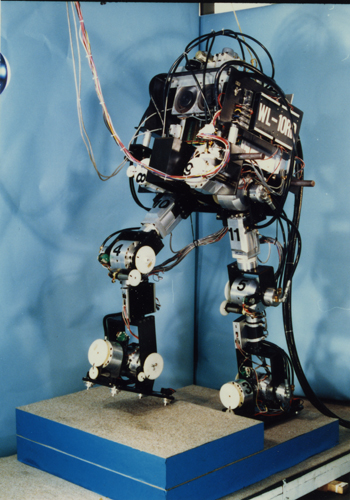
\includegraphics[width=0.8\linewidth]{image46}

    WL-10RD. First dynamic walker using the ZMP scheme (1985).
            \end{center}
        \end{column}
        \begin{column}{0.5\linewidth}
            \begin{center}
                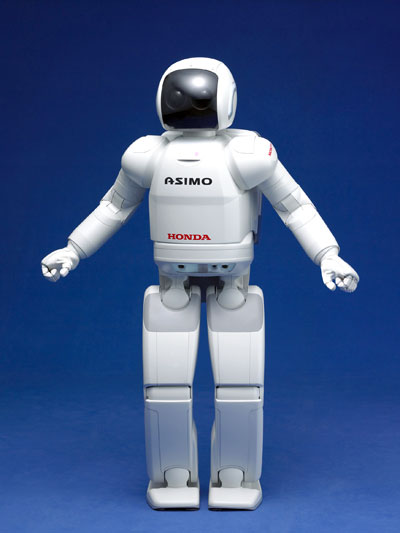
\includegraphics[width=0.8\linewidth]{image47}

    Honda Asimo, uses ZMP scheme for walking as deduced from papers and
    patents(2000-). 
            \end{center}
        \end{column}
    \end{columns}


\end{frame}

\begin{frame}{Requirements of ZMP bipeds}

    The fundamental requirements for ZMP-based walking

    \begin{itemize}

        \item At least six fully actuated joints for each leg: hip (3), knee (1),
            foot (2)
        \item Joint are position controlled (as opposed to speed)
        \item Feet are equipped with force sensors, used to measure ZMP.
    \end{itemize}

\end{frame}

\begin{frame}{Force and moment on a body}

    \begin{itemize}

        \item Resultant force of inertia and gravity forces is
        \item \href{http://en.wikipedia.org/wiki/Moment_of_force}{Moment} (aka
            torque) in any point \emph{X is}

            \[
                M^{gi}_X = \vec{XG} \times mg - \vec{XG} \times ma_G - \dot{H}_G
                \]
    \end{itemize}

    \emph{m} is total mass of robot, \emph{g} is gravitational acceleration
    (9.81 m/s\^{}2), \emph{aG} is acceleration of centre of mass

    is the vector between point \emph{X} and centre of mass \emph{G} and
    \emph{} is rate of
    \href{http://en.wikipedia.org/wiki/Angular_momentum}{angular momentum}
    at \emph{G} ( amount of rotation)

\end{frame}

\begin{frame}{Force and moment because of contact}

    \begin{itemize}

        \item Resultant contact forces
        \item Moment caused by contact forces
    \end{itemize}

    The contact force at a point \emph{C} is given by this equation.

    is the moment at a contact point caused by contact forces

\end{frame}

\begin{frame}{Dynamical balance}

    \begin{itemize}

        \item When forces and moments are opposite the body is dynamically balanced
        \item Zero Moment Point (ZMP)
    \end{itemize}

    \emph{n} is normal vector (a vector perpendicular to a surface of size
    1) to the support surface. \emph{Z} is the Zero Moment Point, P is the
    resultant point of contact of the foot.

    \href{http://ieeexplore.ieee.org/stamp/stamp.jsp?tp=\&arnumber=1325327}{Read
    more here (if you dare)\ldots{}}

\end{frame}

\begin{frame}{ZMP: the problem}

    In theory, it works. In practice, it doesn't always.

    Requires a precise knowledge of where the Centre of Gravity is, what the
    forces are acting on the point of contact, and what the rate of angular
    momentum () of the robot is.

    \begin{itemize}

        \item In practice, this can be done for simple systems (inverted pendulum
            walkers).
        \item Is impossible for real, complex robots.
    \end{itemize}

    \begin{itemize}

        \item ~
    \end{itemize}

\end{frame}

\begin{frame}{Capture steps}

    A promising way forward is to use ``capture steps''.

    \begin{itemize}

        \item A capture step places the foot in the ``capture region'' making the
            robot come to a standstill.
        \item If a robot is \textbf{pushed} it places one foot in the direction of
            the fall.
    \end{itemize}

    If a Capture Point is situated within the convex hull of the foot
    support area (the Base of Support), the robot is able to recover from
    the push without having to take a step. Otherwise, it must take a step.

    NEW

\end{frame}

\begin{frame}[plain]

    \begin{columns}
        \begin{column}{0.5\linewidth}
            \begin{center}
                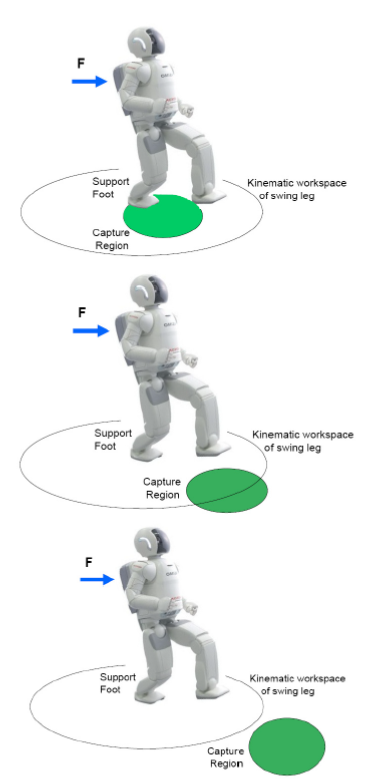
\includegraphics[width=0.8\linewidth]{image56}
            \end{center}
        \end{column}
        \begin{column}{0.5\linewidth}
    \begin{itemize}

        \item The Capture Region intersects the Base of Support, no step is needed.
        \item The Capture Region falls outside the Base of Support, a step is needed
            to prevent falling over.
        \item Same as before, but the Capture Region falls outside the reachable
            space. More than one step is needed to regain balance.
    \end{itemize}
        \end{column}
    \end{columns}

\end{frame}

\begin{frame}{Capture steps examples}

    Fast optimisation of capture steps using a dynamic simulated model

    \begin{itemize}

        \item \href{http://spectrum.ieee.org/automaton/robotics/humanoids/japanese-high-power-humanoid-robot-hrp3l-jsk}{Video}
            and
            \href{http://ieeexplore.ieee.org/xpl/login.jsp?tp=\&arnumber=6100894\&url=http://ieeexplore.ieee.org/xpls/icp.jsp?arnumber\%3D6100894}{paper}
    \end{itemize}

    Walking using capture step

    \begin{itemize}

        \item \href{http://www.ais.uni-bonn.de/movies/WalkingWithCaptureSteps.wmv}{Video}
            and
            \href{http://www.ais.uni-bonn.de/papers/RoboCup_2014_Missura_Capture_Steps.pdf}{paper}
    \end{itemize}

\end{frame}

\section{The hardest problem in robotics?}

\videoframe{figs/part5/asimo.mp4}

\begin{frame}{Why is walking hard for robots?}

    Number of possible gaits is enormous

    \begin{itemize}

        \item Finding a gait that works (a ``robust'' gate) is hard.
        \item One set of parameter settings will typically work for only one type of
            surface under one set of conditions.
    \end{itemize}

    Floor reaction control is very hard

    \begin{itemize}

        \item Human feet sense and change to the structure of the surface. Robots
            don't yet.
    \end{itemize}

    Sensing for walking challenging

    \begin{itemize}

        \item Gyroscopes, accelerometers, cameras, \ldots{} we do not yet understand
            how to use their readings to make robust gaits.
    \end{itemize}

    Power requirements are high

\end{frame}

\begin{frame}{Possible ways forward (1)}

    Closed-loop walking

    \begin{itemize}

        \item Sensors (pressure sensors, IMU, camera, \ldots{}) in a fast loop
            report back on the state of robot, can be used to respond to changes.
        \item Problem 1: measuring on a moving robot is hard.
        \item Problem 2: even if you know what the robot is doing (e.g. falling),
            what to do?
    \end{itemize}

\end{frame}

\begin{frame}{Possible ways forward (2)}

    Letting the robot learn how to walk

    \begin{itemize}

        \item Difficult to do in the ``real world''
        \item Learning or evolving in a physics simulator, and then transferring to
            the real world
        \item Problem: the ``reality gap'' is too big for unstable robot. Can work
            for 2+-legged robots
            (\href{https://www.youtube.com/watch?v=V2ADU8YWIug}{example}), but has
            not been possible yet for bipeds
    \end{itemize}

\end{frame}

\begin{frame}{}
    \begin{center}
        \Large
        That's all, folks!\\[2em]
        \normalsize
        Questions:\\
        Portland Square A216 or \url{severin.lemaignan@plymouth.ac.uk} \\[1em]

        Slides:\\ \href{https://github.com/severin-lemaignan/module-mobile-and-humanoid-robots}{\small github.com/severin-lemaignan/module-mobile-and-humanoid-robots}

    \end{center}
\end{frame}



\end{document}
